\chapter{Machine Learning}
\label{sec:ml}

\section{Boosted Decision Trees}
\label{sec:bdt}

\section{Neural Networks}
\label{sec:nn}

\subsection{Basics}
\label{sec:nn_basics}

\section{Recurrent Neural Networks}
\label{sec:rnn}

Recurrent: If a network has one or more cycles, that is, if it is possible to
follow a path from a unit back to itself.

\subsection{Fully-Connected RNN}
\label{sec:fully_connected_rnn}

Elman network \cite{elman}:
\begin{align}
  c_t &= \sigma_c(W_c x_t + U_c c_{t-1} + b_c) \\
  h_t &= \sigma_h(W_h c_t + b_h)
\end{align}

Elman or Jordan network?

This should be an \emph{Elman} network
\begin{align}
  h_t = \sigma_h(W x_t + U h_{t-1} + b)
\end{align}

Vanishing gradient problem: Applying the sigmoid function multiple times leads
to vanishing gradients (plot?).

\subsection{Long Short-Term Memory}
\label{sec:lstm}

\begin{figure}[t]
  \centering
  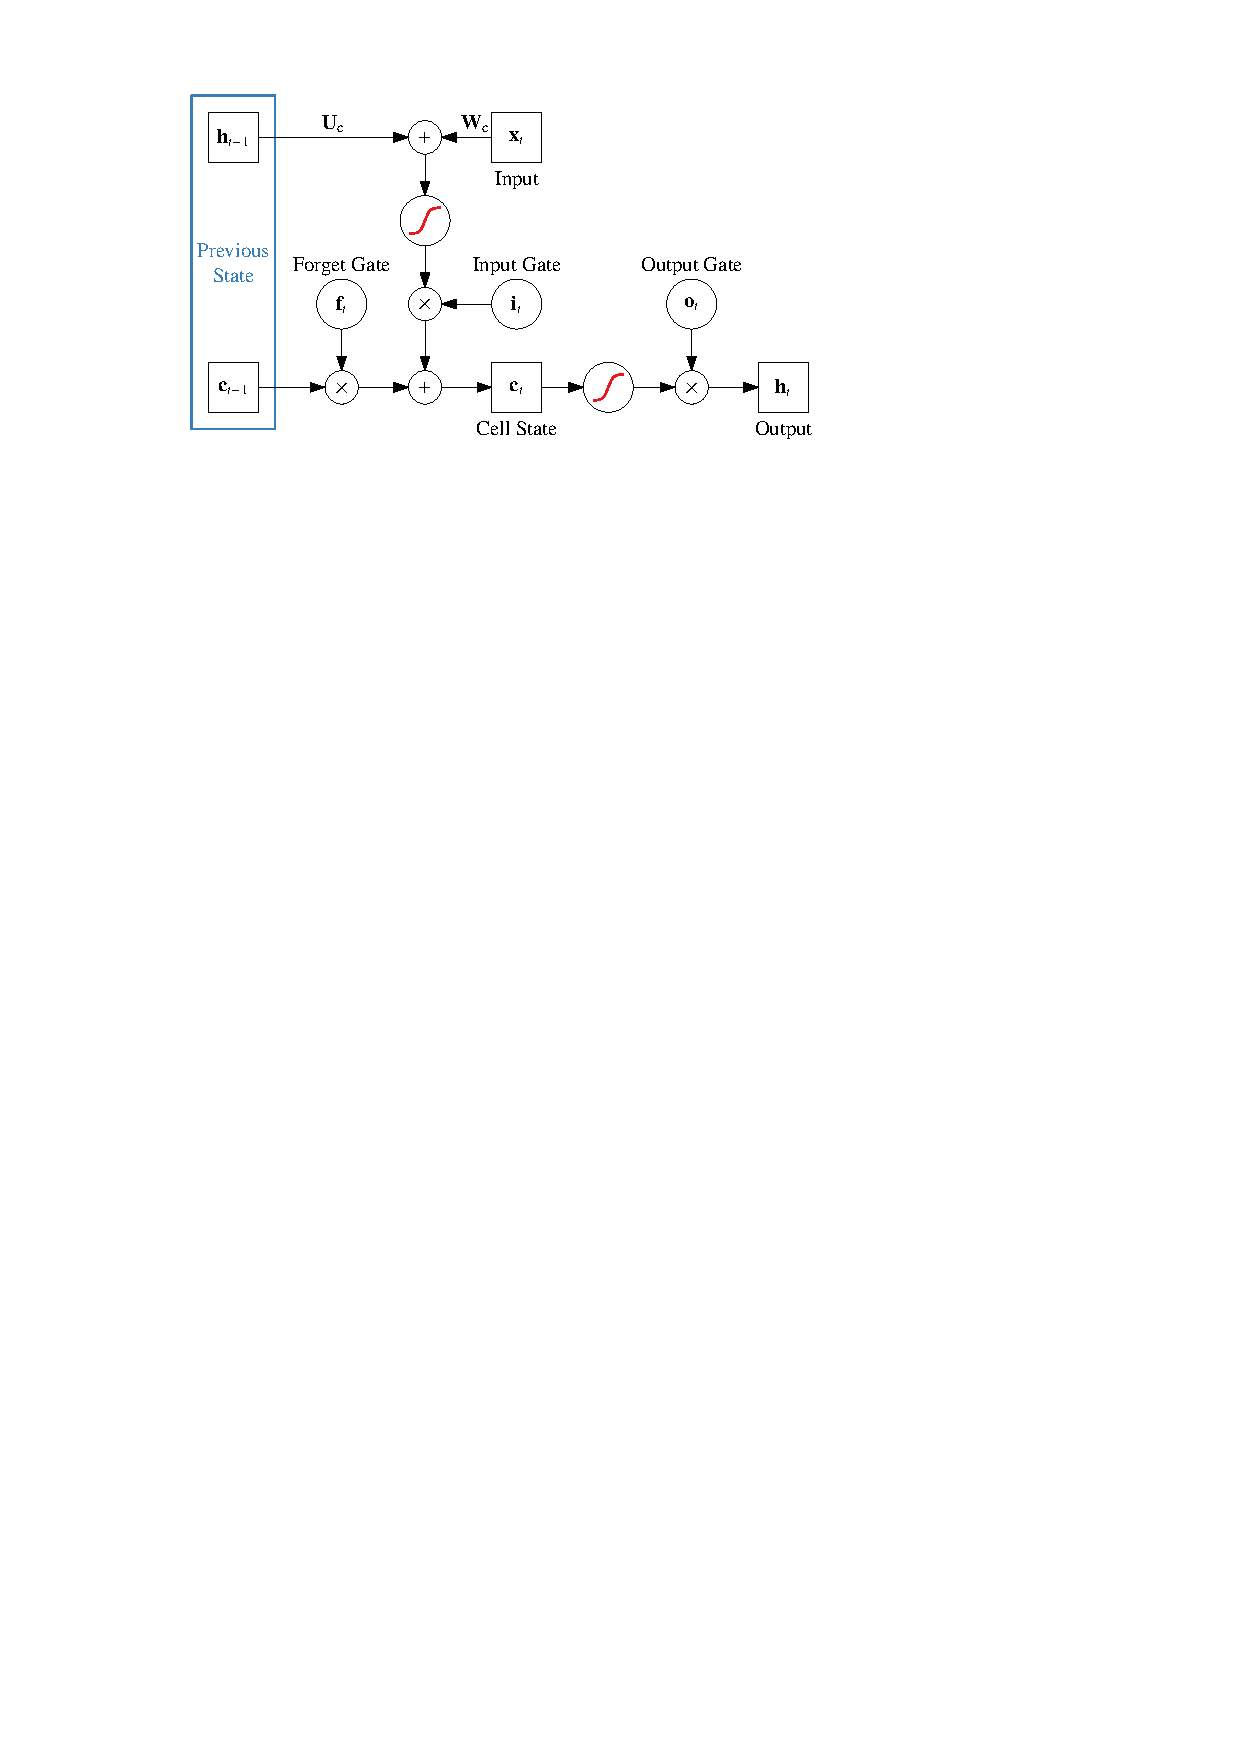
\includegraphics{./figures/theory/LSTM.pdf}
  \caption{Schematic description of a LSTM-cell}
  \label{fig:schematic_lstm}
\end{figure}

\begin{align}
  f_t &= \sigma_g( W_f x_t + U_f h_{t-1} + b_f) \\
  i_t &= \sigma_g( W_i x_t + U_i h_{t-1} + b_i) \\
  o_t &= \sigma_g( W_t x_t + U_o h_{t-1} + b_o) \\
  c_t &= f_t \circ c_{t-1} + i_t \circ \sigma_c(W_c x_t + U_c h_{t-1} + b_c) \\
  h_t &= o_t \circ \sigma_h(c_t)
\end{align}

Stress that the gates depend on $x_t$ and $h_{t-1}$ via learn-able weights.
Therefore the inputting, outputting and forgetting is a learned process.

$\circ$: entry-wise product


Variables:
\begin{itemize}
\item $x_t$: input vector
\item $h_t$: output vector
\item $c_t$: cell state vector
\item $W$, $U$ and $b$: (recurrent -- $U$) weight matrices and bias vector
\item $f_t$, $i_t$ and $o_t$: gate vectors
  \begin{itemize}
  \item $f_t$: forget gate vector
  \item $i_t$: input gate vector
  \item $o_t$: output gate vector
  \end{itemize}
\end{itemize}

Activation functions:
\begin{itemize}
\item $\sigma_g$: element-wise sigmoid function (Gate activation -- recurrent
  activation)
\item $\sigma_c$: element-wise hyperbolic tangent (Cell activation -- recurrent
  activation)
\item $\sigma_h$: element-wise hyperbolic tangent (Output activation)
\end{itemize}

% ------------------------------ FIRST DRAFT ----------------------------- %
This chapter would make sense (Jochen / Will).

\begin{itemize}
\item Own chapter describing the machine learning methods used or include into
  \textit{Theoretical Background}? Alternatively include theory section where
  needed (e.g. have one for the BDT-based studies explaining BDTs [short] and
  one for the RNN studies [longer]).

\item Boosted Decision Trees
  \begin{itemize}
  \item Boosting: Adaptive Boosting $\alpha$, Gradient Boosting $\eta$
  \item Node splitting: Gini Index
  \item Hyperparameters: $N_\mathrm{Trees}$, $d_\mathrm{Tree}$,
  \end{itemize}

\item Neural Networks
  \begin{itemize}
  \item Basics -- focussed on forward pass (Densely connected layers, Activation)
  \item Training -- Weight initialization, Loss functions, Minibatch Gradient
    Descent, Cross-Validation (training, validation, test split)
  \item Recurrent Neural Networks (RNN Equations, Vanishing Gradient Problem,
    Physics Motivation)
  \item Long Short-Term Memory \cite{lstm} (LSTM Equations)
  \item Technical setup (Keras, theano)
  \end{itemize}
\end{itemize}

% -------------------------------- ??? --------------------------------- %

\begin{itemize}
\item Important concepts
  \begin{itemize}
  \item Supervised learning (need truth info)
  \item Overfitting \& train-test split
  \end{itemize}

\item Boosted decision trees
  \begin{itemize}
  \item Boosting (AdaBoost, GradBoost)
  \item Split determination (GiniIndex)
  \item Important hyperparameters
  \end{itemize}

\item (Recurrent) Neural networks
  \begin{itemize}
  \item Layers
    \begin{itemize}
    \item Dense

    \item LSTM (\& Masking)

    \end{itemize}

  \item Frameworks used for this thesis (theano \cite{theano}, keras \cite{keras})

  \end{itemize}

\end{itemize}

%%% Local Variables:
%%% mode: latex
%%% TeX-master: "mythesis"
%%% End:
